\documentclass[twocolumn]{aastex631}

\newcommand{\vdag}{(v)^\dagger}
\newcommand\aastex{AAS\TeX}
\newcommand\latex{La\TeX}
\newcommand{\webb}{JWST}
\newcommand{\jwst}{JWST}
\newcommand{\tess}{TESS}
\newcommand{\mum}{\ifmmode{\rm \mu m}\else{$\mu$m}\fi}
\newcommand{\lightkurve}{{{\fontfamily{lmtt}\selectfont lightkurve}}}
\newcommand{\tesslocalize}{{{\fontfamily{lmtt}\selectfont TESS\_Localize}}}

\shorttitle{TESS Variability of JWST Calibration Stars}
\shortauthors{Mullally et al.}

\graphicspath{{./}{figures/}}

\begin{document}

\title{Searching for TESS Photometric Variability of Possible JWST Spectrophotometric Standard Stars}

\author[0000-0001-7106-4683]{Susan E.\ Mullally}
\affiliation{Space Telescope Science Institute, 3700 San Martin Dr.,
  Baltimore, MD 21218, USA}
\email{smullally@stsci.edu}

\author[0000-0003-4520-1044]{G.~C.~Sloan}
\affiliation{Space Telescope Science Institute, 3700 San Martin Dr., Baltimore, MD 21218, USA}
\affiliation{Department of Physics and Astronomy, University of North
  Carolina, Chapel Hill, NC 27599-3255, USA}

\author[0000-0001-5941-2286]{J.~J.~Hermes}
\affiliation{Department of Astronomy \& Institute for Astrophysical Research, Boston University, 725 Commonwealth Ave., Boston, MA 02215, USA}

\author{Michael Kunz}
\affiliation{Space Telescope Science Institute, 3700 San Martin Dr.,
  Baltimore, MD 21218, USA}
%\affiliation{Howard County High School}

\author[0000-0001-5473-856X]{Kelly Hambleton}
\affiliation{Villanova University, 800 Lancaster Avenue, Villanova, PA 19850, USA}


\author{Scott W. Fleming}
\affiliation{Space Telescope Science Institute, 3700 San Martin Dr.,
  Baltimore, MD 21218, USA}
  
\author[0000-0001-5340-6774]{Karl D.\ Gordon}
\affiliation{Space Telescope Science Institute, 3700 San Martin Dr., Baltimore, MD 21218, USA}

\author{Khalid Mohamed}
\affiliation{Space Telescope Science Institute, 3700 San Martin Dr.,
  Baltimore, MD 21218, USA}
\affiliation{Department of Physics \& Astronomy, Amherst College, C025 Science Center 25 East Drive, Amherst, MA 01002, USA}

\author{Catherine Kaleida}
\affiliation{Space Telescope Science Institute, 3700 San Martin Dr.,
  Baltimore, MD 21218, USA}
  
\author[0000-0001-9806-0551]{Ralph Bohlin}
\affiliation{Space Telescope Science Institute, 3700 San Martin Dr., Baltimore, MD 21218, USA}

\begin{abstract}
We use data from the Transiting Exoplanet Survey Satellite (\tess) to search for, and set limits on, optical to near-infrared photometric variability of the candidate \jwst\ spectrophotometric standards. Our search of 37 of these candidate standards has revealed measurable periodic variability in 15 stars. The majority of those show variability that is less than half a percent; however, four stars are observed to vary photometrically, from minimum to maximum flux, by more than 1\% (the G dwarf \object{HD~38949} and three fainter A dwarfs).  Variability of this size would likely impact the error budget in the spectrophotometric calibration of the science instruments aboard \jwst.  For the 22 candidate standards with no detected variability, we report upper limits on the observed changes in flux.  Despite some systematic noise, all stars brighter than $12^{th}$\,magnitude in the TESS band show a 3$\sigma$ upper limit on the total change in brightness of less than half a percent on time scales between an hour and multiple weeks, empirically establishing their suitability as spectrophotometric standards.


\end{abstract}

\keywords{variable stars, white dwarfs, calibration}


\section{Introduction} 
\label{sec:intro} % Sec. 1.0

The James Webb Space Telescope (\webb), an infrared space telescope with a diameter of 6.5\,m, promises to revolutionize many areas of astrophysics, from exoplanets to the most distant galaxies \citep{Kalirai2018,gardner2006jwst}.  In order to accomplish those goals, \webb\ will observe a sample of spectrophotometric standard stars to calibrate observations across the near- and mid-infrared (0.6--28.8~\mum).  The objective is an accuracy in the observed flux of the standard stars to better than 2\% \citep[see JWST Data Absolute Flux Calibration in][]{jdox}.  A successful standard-star calibration program will not only enable the absolute calibration and the \webb\ cross-instrument calibration, but will also tie \webb\ observations to other space telescopes, such as Hubble, Spitzer, and WISE, and other ground-based observatories as well.

The selection of standard stars must take into account many factors that can reduce both the accuracy and the precision of the spectrophotometric calibration \citep[e.g.][]{Sloan2015}.  The list of possible reasons to reject potential standards during the vetting process is long, but among them, variability is always a red flag.  Variable stars should be avoided because their variations will increase the noise in the calibration data.  Even low-amplitude variability below any level of direct concern could point to more subtle concerns, such as binarity, pulsation, strong magnetic-field activity, or the presence of circumstellar material \citep{Bohlin2014PASP126}. Each of these issues is a reason in itself to reject a candidate, but may have otherwise gone unnoticed.  The identification of any known variable stars prior to their observation by \webb\ will give the calibration team the opportunity to investigate them more closely and potentially save valuable observing time.  Optimizing the calibration of \webb\ will contribute to the success of NASA's flagship mission.

Photometric monitoring of stars, as done by missions like CoRoT \citep{corot}, Kepler \citep{Koch2010} and \tess\ \citep{Ricker2015}, has revealed that they can change brightness due to a variety of factors, and these variations can unexpectedly change in timescale or amplitude. Many of these variations are internal to the star, e.g.\ stellar pulsations or spots rotating in and out of view \citep[e.g.][]{Berger1979deltaScuti, Mcquillan2014}, while other variations are external, e.g.\ eclipses and transits \citep[e.g.][]{prsa2011, Thompson2018}. Time-series photometric observations have revealed many examples of atypical brightness variations where stars change brightness suddenly and in unexpected ways.  For example, Boyajian's star, KIC~8462852, was discovered using Kepler data and shows unexplained drops in the flux of the star as large as 20\% at seemingly random times \citep{Boyajian2016MNRAS}.  The nearby red supergiant Betelgeuse dimmed by more than 1 visual magnitude in 2019, the deepest decline reported in 50-plus years of observations \citep{Betelgeuse2021Natur594,Cotton2020RNAAS4}.  Some white dwarf stars, the classic choice for photometric standards in the UV and optical, have shown both unusual intrinsic variability from pulsations \citep[e.g.][]{Provencal2009ApJGD358,Kilic2015ApJ,Hermes2017MNRAS} and external variability caused by disintegrating planetesimals \citep[as large as 40\%][]{Vanderburg2015Natur,Guidry2021} or accretion disks \citep{Scaringi2021Nat}.  While these examples are rare, they demonstrate that stars can vary for a variety of reasons, many of which are not predictable based on current knowledge.  

\tess\ is well posed to monitor the candidate standards for \webb\ for changes in flux on time scales between minutes and weeks at a precision as fine as a few hundred parts per million \citep{Ricker2015}, an improvement in precision, cadence and coverage over previous observations to identify short term variability in standard stars from the ground \citep[e.g.][]{Marinoni2016}.  \tess\ was launched in 2017 with the purpose of identifying transiting exoplanets around nearby stars.  It photometrically observes a swath of sky covering 24 degrees by 90 degrees for a month at a time and has a bandpass of 0.6--1~\mum\ \citep{Ricker2015} that overlaps with the shortest wavelengths of the \webb\ bandpass.

As a result, \tess\ has serendipitously observed most of the candidate spectrophotometric standards for \webb\ over the course of its mission, and it will continue to do so in its extended mission.  We have examined the \tess\ data for these candidates, looked for evidence of photometric variability, and we report upper limits on any variability if none was detected.  For the 15 \jwst\ spectrophotometric standards found to show statistically significant periodic variability, we show a light curve and periodogram, and provide a few simple statistics describing the amplitude of the variations. 

%Finally, we discuss the limits of this analysis and suggest future observations that could be used to further monitor these potential spectrophotometric standard stars crucial to get the most absolute precision from \jwst\ observations.


\section{Candidate JWST Spectrophotometric Standard Stars} 
\label{sec:targets}

Spectrophotometric calibration requires accurate models of the stars chosen as standards, because any errors in the assumed true spectrum of a standard will propagate into the entire calibrated database \citep{Gordon2022inprep}.  Calibrating with a sample of standards will reduce the impact of problems with the model of any one star, and combining different types of standards will reduce the problems even further.  By comparing the calibration as determined from different stars, and different classes of stars, outliers can be identified and their models corrected, or, if that proves impossible, the stars can be rejected.

The \webb\ calibration will be based on three classes of standard stars:  white dwarfs, A dwarfs, and solar analogs (i.e., G dwarfs) \citep{Gordon2022inprep}.  It is expected that five stars of each class will be observed during the \jwst\ mission to accomplish this task.  Comparisons of the stars will identify potential issues with models of the stars and possible outliers.  The sample examined in this paper, see Table~\ref{tab:targets}, is based on lists of candidates available in the JWST User Documentation accessed in 2020~December \citep{jdox}.  It must be stressed that the candidate list is evolving as stars are vetted and new stars are added to better cover parameter space \citep{Gordon2022inprep}.  The calibration standard stars in this list overlap calibration stars used by other observatories. For example, the list includes A dwarf stars reported by \citet{Reach2005} to be primary standards for IRAC on Spitzer (see those with shortened-names starting with J in Table~\ref{tab:targets}). For more information on how the calibration stars are selected, see \citet{Gordon2022inprep}.


%The calibration standards observed by the Hubble and Spitzer Space Telescopes form the basis of the list of candidates.  Bright stars have been added for the mid-infrared calibration, along with faint ones to probe dynamic range. 

%Note, if you make changes to the information in this table, it need to be propogated
%Back to the original data file, so let Susan know.
\startlongtable
\begin{deluxetable*}{lrcrcr} % Table 1
\tablecolumns{6}
\tablewidth{0pt}
\tablecaption{Candidate standard star properties with TESS data. }
\tablehead{
  \colhead{Target Name } & \colhead{TIC ID}  & \colhead{Class} & \colhead{T}& 
  \colhead{Cadence}& \colhead{Coord.}\\
  \colhead{} & \colhead{} & \colhead{}& \colhead{[mag]}& \colhead{min} & \colhead{J2000}
}
\startdata
GSPC P330-E &   8591766 & \textbf{(G0 V)} & 12.4 &  30  & 16 31 34  +30 08 46  \\
   16 Cyg B &  27533327 &         G3 V &  5.6 &   2  & 19 41 52  +50 31 03  \\
   HD 38949$^a$ &  32869782 &         G1 V &  7.3 &   2  & 05 48 20  $-$24 27 50  \\
    HD 6538 &  39464221 &         G1 V &  5.9 &   2   & 17 32 01  +34 16 16  \\
  $\eta^1$\,Dor &  41232189 &         A0 V &  5.8 &   2   & 06 06 09  $-$66 02 23  \\
      $\mu$ Col & 100589904 &       O9.5 V &  5.5 &   2  & 05 46 00  $-$32 18 23  \\
     10 Lac & 128692445 &         O9 V &  5.1 &   2   & 22 39 16  +39 03 01  \\
   HD 37962 & 140282069 &         G2 V &  7.2 &   2    & 05 40 52  $-$31 21 04  \\
WD 1057+719 & 147921014 &        DA1.2 & 15.1 &   2    & 11 00 34  +71 38 03  \\
     GD 153 & 149505899 &        DA1.2 & 13.7 &   2    & 12 57 02  +22 01 53  \\
  HD 116405 & 165370459 &         A0 V &  8.4 &   2    & 13 22 45  +44 42 54  \\
     HR 701 & 166698220 &         A5 V &  5.7 &   2    & 02 22 55  $-$51 05 32  \\
  HD 101452 & 181240911 & \textbf{(A9 V)} &  7.3 &   2    & 11 40 14  $-$39 08 48  \\
    HR 6514 & 198456033 &         A4 V &  6.4 &   2    & 17 26 05  +58 39 07  \\
   J1757132$^*$ & 219094190 & \textbf{(A9 IV)} & 11.6 &  30    & 17 57 13  +67 03 41  \\
GSPC P041-C$^b$ & 219015049 &       (G0 V) & 11.5 &   2    & 14 51 58  +71 43 17  \\
   J1808347$^*$ & 219114641 &       (A3 V) & 11.9 &   2    & 18 08 35  +69 27 29  \\
 BD+60 1753 & 219752116 &         A1 V &  9.7 &   2    & 17 24 52  +60 25 51  \\
  HD 163466 & 219820925 & \textbf{(A7 V)} &  6.7 &   2    & 17 52 25  +60 23 47  \\
   J1732526$^*$ & 219897252 &       (A4 V) & 12.5 &   2    & 17 32 53  +71 04 43  \\
  HD 180609 & 229945862 & \textbf{(A3 V)} &  9.3 &   2    & 19 12 47  +64 10 37  \\
  HD 115169$^c$ & 229980646 &         G3 V &  8.7 &   2    & 13 15 47  $-$29 30 21  \\
   J1802271$^*$ & 233067231 &       (A2 V) & 12.0 &   2    & 18 02 27  +60 43 36  \\
   J1805292$^*$ & 233075513 & \textbf{(A3 V)} & 12.2 &   2    & 18 05 29  +64 27 52  \\
   J1812095$^*$ & 233095291 &       (A3 V) & 11.6 &   2    & 18 12 10  +63 29 42  \\
   J1743045$^*$ & 233205654 & \textbf{(A8 V)} & 13.3 &   2    & 17 43 04  +66 55 02  \\
      GD 71 & 247923021 & \textbf{DA1.5} & 13.4 &   2    & 05 52 28  +15 53 13  \\
    HR 5467 & 298165335 &         A1 V &  5.8 &   2    & 14 38 15  +54 01 24  \\
   G191-B2B & 327587572 &        DA0.8 & 12.2 &   2    & 05 05 31  +52 49 52  \\
  HD 167060 & 365653206 &         G3 V &  8.4 &   2    & 18 17 44  $-$61 42 32  \\
     $\delta$ UMi & 383553764 &       A1 Van &  4.4 &   2    & 17 32 13  +86 35 11  \\
    HR 7018$^d$ & 383676357 &         A0 V &  5.8 &   2    & 18 37 34  +62 31 36  \\
GSPC P177-D & 417544924 & \textbf{(G0 V)} & 12.9 &  30    & 15 59 14  +47 36 42  \\
   HD 55677 & 440765193 &         A2 V &  9.4 &  10    & 07 14 31  +13 51 37  \\
  HD 205905$^e$ & 441120034 &    G1.5 IV-V &  6.2 &   2    & 21 39 10  $-$27 18 24  \\
   $\lambda$ Lep & 442871031 &      B0.5 IV &  4.6 &   2    & 05 19 35  $-$13 10 36  \\
 WD1657+343 & 471015233 &        DA0.9 & 15.8 &   2    & 16 58 51  +34 18 53  \\
\enddata

\tablecomments{Spectral types in parenthesis are not optical spectral classifications and instead are based on photometry and/or spectra from STIS on Hubble.  References for the spectral types are the same as those specified by \citet{Gordon2022inprep}. References for the remaining spectral types is as follows: $^a$\citet{Houk1988mcts}, $^b$\citet{Bohlin2011AJ}, $^c$\citet{Houk1982mcts-hd115169}, $^d$\citet{Crowley1969AJ}, $^e$\citet{Keenan1989ApJS}. \newline
$^*$ Stars with names beginning with 'J' are Spitzer standards described in \citet{Reach2005} and as done their are given shortened names based on the 2MASS designation. J1757132 is 2MASS~J17571324+6703409. J1802271 is 2MASS J18022716+6043356. J1732526 is 2MASS~J17325264+7104431.  J1805292 is 2MASS~J18052927+6427520. J1808347 is 2MASS J18083474+6927286. J1812095 is 2MASS~J18120957+6329423. J1743045 is 2MASS~J17430448+6655015.}
\label{tab:targets}
\end{deluxetable*}


\section{TESS Observations}
\label{sec:obs}
%DOI: 10.17909/t9-tkr5-6a83 
%Dataset Title: JWST Spectrophotometric Standard Candidates

To study the variability of the candidate spectrophotometric standards, we use observations from \tess\ spanning Sectors 1 to 40, which spans the years 2017--2021. When possible, we utilize the 2-minute cadence data processed by the Science Processing Operations Center (SPOC) pipeline, which provides high-quality background subtraction, systematic correction and flux-dilution corrections due to the large pixel scale of \tess\ \citep{kdph2020ksciApertures,kdph2020ksciCal,kdph2020ksciPA,kdph2020PDC}. A few of our candidate stars were only observed by \tess\ in the Full Frame Images (FFIs). For these targets, we only report on their variability if MAST hosts \tess-SPOC high-level science products \citep{Caldwell2020spoc}, since these are similarly processed by the SPOC pipeline and have corrections applied for crowding due to the large \tess\ pixels. These FFIs collect data on the stars at either a 30-minute or 10-minute cadence, depending on whether or not the data were collected after the second year of the \tess\ mission. See Table~\ref{tab:targets} for a list of those targets used in our analysis, including their TESS Input Catalog (TIC) identification and magnitude \citep{Stassun2018TIC}. All of the data is available at MAST: DOI~ \dataset[10.17909/t9-tkr5-6a83]{\doi{10.17909/t9-tkr5-6a83}}.

Regardless of the observed cadence, we used the pre-search data conditioned, simple aperture photometry (PDCSAP) photometric time series (see \citealt{Smith2012,Stumpe2012PASP} for details on the PDCSAP processing steps). As an overview, the TESS pipeline that creates these light curves removes the background, performs simple aperture photometry using a fixed aperture that optimizes the signal-to-noise of the light curve, and then removes systematics by fitting Principal Component Analysis (PCA) basis vectors that represent common signals observed in nearby stars. 

We then use the software \lightkurve\ \citep{lightkurve} to detrend, and normalize the light curve. For some light curves we further removed obvious systematic variations by applying a Savitzky-Golay filter \citep{savgol1964AnaCh..36.1627S} with a window length of half of the number of data points in the sector. As a sector is $\approx$27 days long, we only expect to be able to unequivocally measure variability with time scales shorter than half the length of the sector ($\approx 13$\,days).  Variability longer than this time scale, unless very large in amplitude, is often mistaken for systematics and is commonly removed from the time series. While \tess\ data can be used to find longer-period trends, it requires very careful examination of possible systematic noise and stitching together consecutive sectors of data. For this study we restrict our analysis to repeatable variability of time scales shorter than $\approx 13$\,days in length and large-amplitude, single-occurrence variations (such as eclipses or flares).

To look for periodic variations, we used Lomb-Scargle periodograms \citep{Lomb1976,lightkurve} and report those with significant peaks that otherwise do not appear to be caused by systematic noise (see Section~\ref{sec:var}).  For those with no significant variability, we provide upper limits to any variability that could be detected (see Section~\ref{sec:novar}).

%We also examined the light curve for each sector by eye to look for any large, single-occurrence outliers in the relative flux that could not be explained by systematic noise. None of the light curves we examined showed evidence of flares, transits, eclipses or other transient, short-duration events that were not more readily explained by systematic noise.

\subsection{Stars with Variability}
\label{sec:var}

We found 15 of the \webb\ spectrophotometric standards stars in our sample to have statistically significant periodic variability. Only four show variability in flux larger than 1\% when considering the full extent of the observed variability (minimum to maximum brightness, or peak-to-peak).  For each variable star, the largest peak in the periodogram is highly significant and is at least 5 times larger than the noise level of the periodogram \citep{KjeldsenBedding1995, Baran2021}. Figures~\ref{fig:lcft1} -- \ref{fig:lcft4} show parts of the light curve and Lomb-Scargle periodogram created from one entire \tess\ sector for the 15 variable stars in our sample (two sectors for the case of HD~38949). 
Figure~\ref{fig:lcft1} highlights the four with the largest variations.  
%For all of these stars at least one observed peak in the periodogram is five times the noise level (calculated as described in Appendix A of \citet{KjeldsenBedding1995}).

Table~\ref{tab:variable} summarizes the amplitude of the variations and their approximate period.  It lists the period of the maximum amplitude peak along with the maximum amplitude. Since most stars have more than one period of variability, the maximum amplitude in the periodogram does not capture the full change in relative flux observed in the \tess\ light curves. To approximate full observed peak-to-peak variability in the presence of noise, we calculate the quantity $V_{95}$, which is defined to be the difference between the maximum and minimum values of those points contained by 95.45\% of the values in the light curve centered on the median.  $V_{95}$ measures the envelope of all data within $\pm 2\sigma$ of the median. 

%Dividing that quantity by four is approximately the same as the standard deviation of the light curve. -- Not true except in a few cases because there is a non-gaussian signal there. 

When reporting the statistics we use the sectors shown in Figures~\ref{fig:lcft1} -- \ref{fig:lcft4} and bin the light curves to 6-minute bins to improve the signal-to-noise ratio in some of the dimmer stars. The displayed sectors were chosen to be representative of the observed variability and have the lowest observed noise. The $V_{95}$ statistic acts as a reasonable measure of the full amplitude of the observed variability for those whose amplitudes are significantly larger than the noise.  For the fainter stars with low amplitudes and noisy light curves, $V_{95}$ overestimates the true extent of the observed variability. No single statistic will fully summarize the variability of these stars; the light curves and periodograms provide a more complete picture of the  amplitude and shape of the periodicity.

A single \tess\ pixel covers more than 21 arc seconds of the sky on a side, making it possible for nearby sources to contaminate our light curves. Table~\ref{tab:variable} also includes the crowding metric calculated by the SPOC pipeline, as a way to quickly asses the impact of nearby sources. The crowding metric indicates the fraction of the light in the aperture that comes from the target star given the positions and amplitudes of stars in the TIC.  A value near 1.0 indicates an isolated star, while lower values indicate significant crowding from neighbors.  Two of our large-amplitude variables (J1732526 and J1812095) have crowding values around 0.8.  The SPOC Pipeline corrects the light curve amplitudes for any dilution due to nearby stars by using this crowding value \citep{FausnaughDRN}.  As a result, the amplitudes and upper limits we report in this paper have already accounted for these neighbors.

% J1732526 = TIC 219897252
% J1812095 = TIC 233095291

Due to the presence of nearby stars for two of our large variables, we investigated the false positive scenario that one of the nearby stars is varying instead of the target of interest. To test this possibility, we use the code \tesslocalize\ \citep{HiggensBell} to determine if the location of the observed variations in the pixel time series is consistent with the position of the target star, as reported by Gaia Data Release 2 \citep{gaiaDR22018}.  We do this analysis on the large amplitude frequencies from Sector~40 data for both J1732526 and J1812095. The per pixel amplitude heat maps shown in Figure~\ref{fig:cent} for J1732526 were calculated using the five largest frequencies and the two largest frequencies for J1812095 apparent in the periodogram.  These per pixel amplitudes are then fit to the \tess\ pixel response function (PRF) to obtain the true location of the variability. In both cases the location on the CCD of the largest amplitudes overlaps with our target star.  For completeness, we performed the same analysis on all 15 variable stars, despite having no bright, nearby sources. In no case did evidence emerge that a nearby source caused the variations, though for many stars with less significant variability, it was not always possible to convincingly extract and fit per pixel variability.


\begin{deluxetable*}{lllcrcc}
\tablecolumns{6}
\tablewidth{0pt}
\tablecaption{Candidate spectrophotometric standards with observed variability.}

\tablehead{
  \colhead{Target Name} & \colhead{TIC ID} & \colhead{Class} & \colhead{CROWD$^{\dagger}$} & \colhead{Period} & \colhead{max Amp.} & \colhead{$V_{95}$} \\
  \colhead{} & \colhead{} & \colhead{} & \colhead{} &\colhead{[days]}& \colhead{[\%]}& \colhead{[\%]}
}
\startdata
 \object{HD 38949} &  32869782 &    G1V &    0.998 & 3.798 & 0.284 & 1.17 \\
\object[eta01 dor]{$\eta^1$\,Dor} &  41232189 &    A0V &    1.000 & 0.249 & 0.037 & 0.18 \\
   \object{$\mu$ Col} & 100589904 &    O9V &    0.999 & 1.196 & 0.024 & 0.12 \\
   \object{HR 701} & 166698220 &    A6V &    1.000 & 0.845 & 0.005 & 0.05 \\
 \object{HR 6514} & 198456033 &    A3V &    1.000 & 0.054 & 0.058 & 0.42 \\
 \object[2MASS J18083474+6927286]{J1808347} & 219114641 &    A3V &    0.991 & 0.026 & 0.419 & 1.65 \\
\object{HD 163466} & 219820925 &    A6V &    1.000 & 0.101 & 0.064 & 0.17 \\
 \object[2MASS J17571324+6703409]{J1732526} & 219897252 &    A3V &    0.831 & 0.020 & 0.178 & 1.40 \\
 \object[2MASS J18120957+6329423]{J1812095} & 233095291 &    A3V &    0.780 & 2.442 & 0.396 & 1.57 \\
  \object{HR 5467} & 298165335 &    A1V &    1.000 & 0.995 & 0.004 & 0.05 \\
 \object[del umi]{$\delta$ UMi} & 383553764 &    A1V &    1.000 & 0.761 & 0.004 & 0.04 \\
  \object{HR 7018} & 383676357 &    A0V &    0.996 & 2.547 & 0.029 & 0.13 \\
 \object{HD 55677} & 440765193 &    A4V &    0.984 & 0.145 & 0.029 & 0.24 \\
\object{HD 205905} & 441120034 &    G2V &    0.999 & 9.986 & 0.068 & 0.26 \\
 \object[lam Lep]{$\lambda$ Lep} & 442871031 &  B0.5V &    1.000 & 1.260 & 0.148 & 0.35 \\
\enddata

\tablecomments{The column Period gives the period of the largest amplitude peak (max Amp.) seen in the periodogram. $V_{95}$ is the peak-to peak range encompassing 95.45\% of the binned observed relative fluxes. Errors on the max Amp. value are less than 0.002\% with the exception being the 'J' stars ($T_{mag}\ge11$) whose errors are near 0.01\%.
\\
$^{\dagger}$CROWD comes from the CROWDSAP estimate from the \tess\ SPOC pipeline and is the fraction of flux from the target in the extracted aperture.}
\label{tab:variable}
\end{deluxetable*}
\vspace{-1em}

\begin{figure*}
\centering
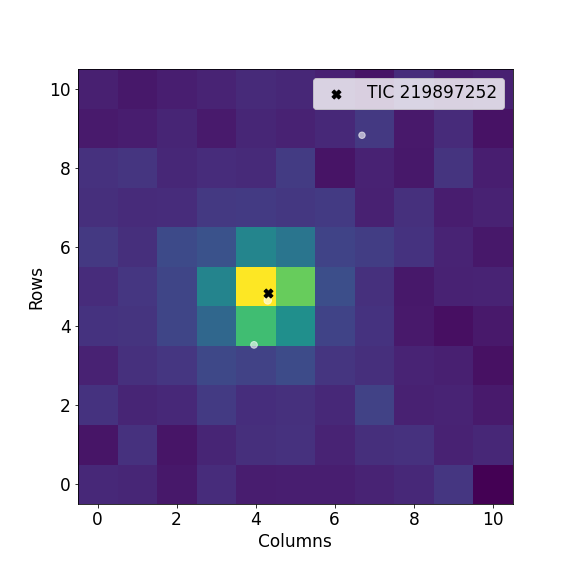
\includegraphics[width=0.45\linewidth]{figures/TIC219897252_s040_5modes_tloc.png}
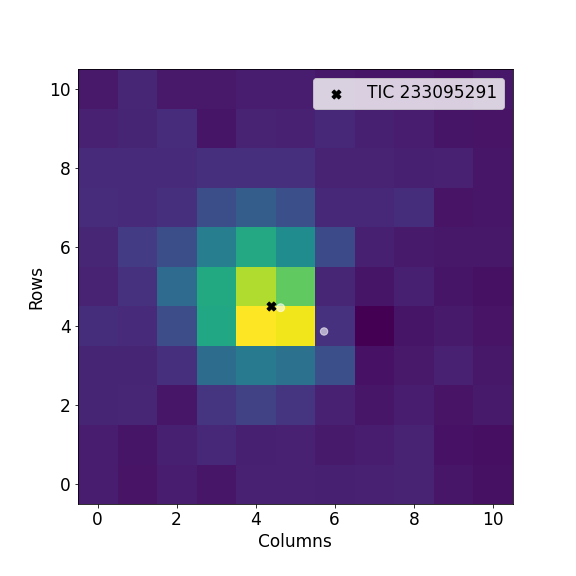
\includegraphics[width=0.45\linewidth]{figures/TIC233095291_s040_2modes_tloc.png}
\caption{Pixel heat maps of the fitted amplitudes at the specified periods across the pixels downloaded from \tess\ in Sector 40 as generated by \tesslocalize\ \citep[][]{HiggensBell}. TIC 219897252 is on the left and TIC 233095291 is on the right. The grey circles represent known Gaia Data Release 2 sources with $T_{mag} > 15$, three magnitudes dimmer than the target stars. The black 'x' represents the best fit between the heat map and the \tess\ PRF. In both cases the best fit location overlaps the Gaia location of our target at the center of the \tess\ pixels, indicating that the variability comes from the targeted source.} 
\label{fig:cent}
\end{figure*}

\subsection{Reasons for Variability}

While we do not attempt to definitively explain the physical reasons for the variability we observe in these stars, it is likely the reason for the photometric variability is related to either stellar pulsations or spots. 

May of our variable stars are A-dwarf stars.  Variability in A-type stars can occur due to a plethora of reasons, including stellar pulsations.  The $\delta$ Scuti variables appear at the intersection of the instability strip and the main sequence \citep[e.g.,][]{Petit1987}.  They are the most prominent pulsators among A dwarfs, and they make up $\sim$27\% of all variable A and F dwarfs \citep{Uytterhoeven2011}.   They pulsate in pressure modes and mixed pressure and low-order gravity modes due to the $\kappa$ mechanism \citep{Lee1985}, with pulsation frequencies in the range 18\,min to 8\,hrs \citep{Amado2004}. $\gamma$ Doradus variables also appear in a similar part of the HR diagram \citep[e.g.,][]{Kaye1999}, although they are rarer than $\delta$ Scuti stars, making up $\sim$12\% of all variable A and F dwarfs. \citep{Uytterhoeven2011}. $\gamma$ Dor variables pulsate in non-radial, high-order gravity modes caused by convective blocking \citep{Guzik2000} with pulsation periods typically on the order of one day \citep{Grigahcene2010}.  Some stars, known as hybrid $\gamma$ Dor-$\delta$ Scuti stars, exhibit both $\gamma$ Dor and $\delta$ Scuti pulsations \citep{Grigahcene2010}.  These hybrid pulsators account for an additional $\sim$23\% of all variability found in A and F dwarfs. In our sample we find evidence of all three types of the above pulsators at varying amplitudes.

Other than pulsations, binarity and rotational modulation due to spots can also cause variations in A stars. In our sample, we do not find evidence of short-period, eclipsing binarity which is expected since these usually have large flux variations that would have been seen in previous observations. Regarding rotation, \citet{Balona2013, Balona2017} claim to have found spots in more than 50\% of A stars in the Kepler data, suggesting that modulation due to surface rotation is more commonly observed than previously thought. However, the origin of spots in A and B stars is currently under debate, as these stars do not have a significant surface convective zone, which is usually associated with surface spots. The presence of a fossil magnetic field \citep{Parker1955} and the creation of a magnetic field caused by a dynamo effect in mass motions that occur in convective layers \citep{Charbonneau2014} are two of the contending ideas for the creation of spots in hotter main sequence stars. In our sample, we find signatures that suggest the presence of spots in several objects:  HD 38949, J1812095, $\lambda$~Lep, eta01~Dor and HR~7018.



\subsection{Largest Variable Stars}

In this section we discuss in more detail the size and astrophysics for the variability of the six stars with the largest changes in brightness that we measured in the \tess\ data from our target list. Each of these stars show a $V_{95}\ge0.35$\%. In these cases, the time scale and amplitude of the variations, could impact high precision spectrophotometric calibrations, and their variability should be considered before using them as a standard star. The remaining 9 stars have small enough amplitudes that at least for JWST they will not have significant impact on the calibrations. 

Three of the large amplitude variable stars are A dwarf stars from the \citet{Reach2005} Spitzer calibration. The amplitudes we see here were likely below the level of detection for Spitzer. For comparison, \citet{Krick2021IRAC} measured the IRAC fluxes in dozens to thousands of observations for most of our variable stars and reported standard deviations between 0.7\%\ and 2.8\%\ for the 3.6$\mu m$ band.  This observed scatter is approximately 4 times larger than the variability we report here.


\subsubsection{HD~38949 (TIC~32869782)}

This G dwarf varies with a peak-to-peak amplitude of 1.2\% (see top panel of Figure~\ref{fig:lcft1}). \tess\ observed HD~38949 in Sectors 6, 32, and 33.  The power spectrum is complex and shows a 7.9\,day peak along with peaks at both a half and quarter of that period. This quasi-periodic, oscillatory behavior is consistent with a combination of stellar rotation at a 7.9\,day period and migrating star spots on the surface due to strong magnetic activity \citep{Santos2021}.  HD~38949 is also an x-ray source, as revealed by the Swift Observatory \citep{Swift2020,Evans2020vizier}, which supports a picture of active spots and flares. Due to these properties, the \jwst\ calibration team has already removed this star from the list of standards \citep{Gordon2022inprep}.

It is also noteworthy that HD~38949 is listed in the HST CALSPEC database  \footnote{\url{https://www.stsci.edu/hst/instrumentation/reference-data-for-calibration-and-tools/astronomical-catalogs/calspec}} \citep{Bohlin2014PASP126}, as a star with complete STIS coverage that could be used to support flux calibrations of other observatories.


%HD~38949 is a known standard starDue to these properties, this star has already been removed from lists of standards for \webb (private communication).
% ($T_{mag}=$7.3) 
% SWIFT - IX/58/2sxps - 2020yCat.9058....0E
% only X-ray source among the solar analogs in the sample

\subsubsection{J1808347 (TIC~219114641)}

This A dwarf shows a rich set of peaks in its periodogram that produce a peak-to-peak amplitude of 1.65\% (see second panel in Figure~\ref{fig:lcft1}). These large variations  make it a poor spectrophotometric standard. The periods range from 0.5 to 1.0 hours, with the strongest mode at 0.6 hours.  The high frequency variations are caused by $\delta$ Scuti pulsations.  The variability is difficult to see in the 30-minute \tess\ data taken during the first year of TESS observations; however, they are more apparent in the 2-minute cadence data from Sectors 40 and 41.  This star will be observed again by \tess\ in Sectors 47--55.  

%The large-amplitude ($>1$\%) flux variations observed in \tess\ will likely prevent this target from being considered a suitable target for high precision calibrations, like those required for \webb.




\subsubsection{J1732526 (TIC~219897252)}

J1732526 is an A star that behaves much like J1808347; it is multiperiodic, with its strongest mode having a period of 0.5 hours, suggesting most of the variability arises from $\delta$ Scuti pulsations (see third panel in Figure~\ref{fig:lcft1}). Its light curve has a peak-to-peak amplitude of roughly 1.4\%, making it a poor spectrophotometric standard. However, in this case, this statistic is somewhat inflated by the inherent noise of this $12.5$ mag object. The combined amplitudes of the largest peaks point to a peak to peak variation closer to 1\%.  In addition to the roughly 0.5-hour pulsation modes, the light curve also shows a longer-period component (roughly 2.5 days). This latter component could arise from rotation, or it could indicate that J1732526 is a hybrid $\delta$ Scuti ($p$-mode) -- $\gamma$ Doradus ($g$-mode) pulsator. \tess\ observed this star at a 2-minute cadence in Sectors 40 and 41 and is planning to observe it again in Sectors 48--55.


\subsubsection{J1812095 (TIC~233095291)}

This A dwarf ($T_{mag}=$11.6) shows consistent oscillations with periods of 1--3\,days and peak-to-peak changes in the flux greater than 1.5\% in the TESS bandpass (see bottom panel in Figure~\ref{fig:lcft1}).  The light curve and periodogram shows significant, though somewhat inconsistent variations at a period of 2.44 days, with a secondary peak at exactly half that period, which is indicative of rotational modulation due to spots.  The periodogram shows no evidence for short-period peaks (i.e., for periods of an hour or less).  \tess\ observed this star in Sectors 14--26 at a 30-minute cadence, and at a 2-minute cadence in Sector 40.  The variability is approximately the same across all sectors. The large peak-to-peak variability on long time scales may make this target not suitable for high-precision spectrophotometric calibration studies.

%J1812095 was one of 11 stars reported as primary standards for IRAC on Spitzer by \cite{Reach2005}.  They did not report any variability, but it may have been below their detection limit.  


\subsubsection{HR~6514 (TIC~198456033)} % HD 158458

The periodogram of this bright A dwarf ($T_{mag}=6.4$) shows a complex set of peaks with periods between roughly 0.5 and 2.0 hours (see top panel of Figure~\ref{fig:lcft2}).  The strongest mode has a period of 1.3 hours.  The periodicity is too fast to arise from stellar rotation and thus likely arises from short-period, likely $\delta$ Scuti ($p$-mode) pulsations.  \tess\ observed this star in Sectors 14--26 and 40--41, and is expected to observe it again in Sectors 47--55.  In the present data, the variability is consistent in amplitude from one sector to the next. 

%The total size of the variability of the light curve is just above 0.4\%, which may not be large enough to outright remove it from the \webb\ calibration list.  The variations, however, do indicate surface temperature changes from pulsations that might compromise this star as a spectrophotometric standard.



\subsubsection{$\lambda$ Lep (TIC~442871031)}

This B9.5 dwarf ($T_{mag}=$4.6) varies with a coherent period of 1.26\,days and multiple exact harmonics of this base period, which suggests that the variation is due to spots on the stellar surface. The peak-to-peak amplitude greater than 0.3\% (see the fourth panel of Figure~\ref{fig:lcft2}). \tess\ observed this star in two sectors: 5 and 32. In both sectors the variability was similar in amplitude and shape. $\lambda$ Lep is one of the hot B dwarfs under consideration for use as standards starting in \jwst\ Cycle 2 \citep{Gordon2022inprep}. 
%The amplitude of the variation is small enough that it could still be considered a suitable standard star for \webb. 



\begin{figure*}
    \centering
    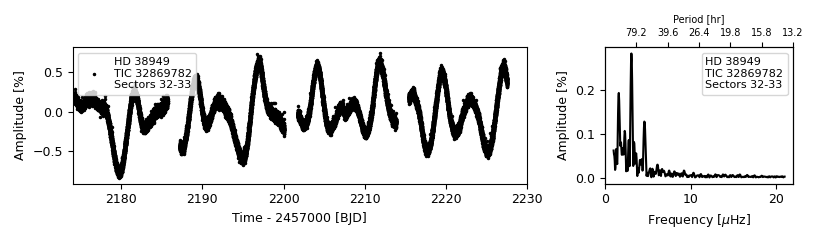
\includegraphics[width=0.9\linewidth]{figures/tic00000032869782_s323_norm1.fits.png}
    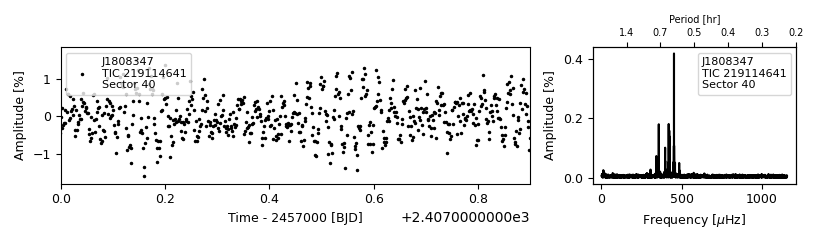
\includegraphics[width=0.9\linewidth]{figures/tic00000219114641_s040_flat2.fits.png}
    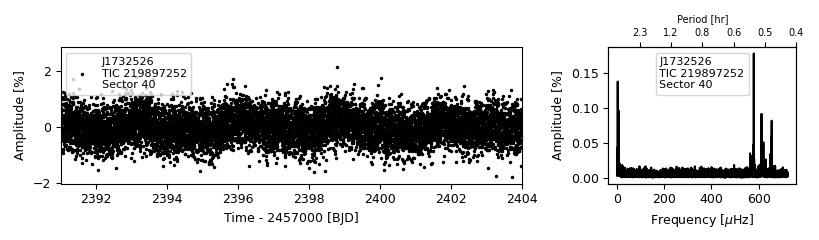
\includegraphics[width=0.9\linewidth]{figures/tic00000219897252_s040_norm1.fits.png}
    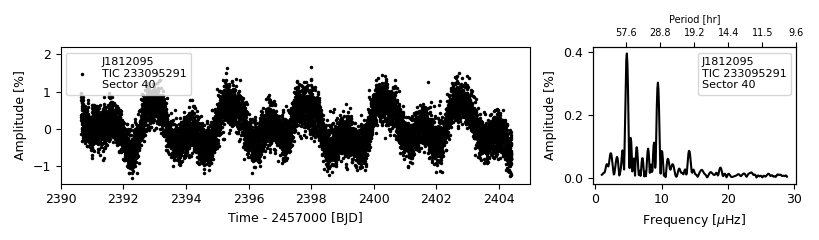
\includegraphics[width=0.9\linewidth]{figures/tic00000233095291_s040_flat1.fits.png}
    \caption{Light curve (left) and periodogram (right) of stars with peak to peak detected variability larger than approximately half a percent. The \tess\ sector(s) used to generate both are labeled on each plot.}
    \label{fig:lcft1}
\end{figure*}

\begin{figure*}
\centering
    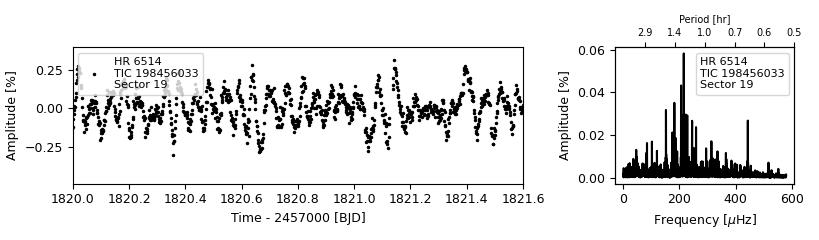
\includegraphics[width=0.9\linewidth]{figures/tic00000198456033_s019_norm1.fits}
    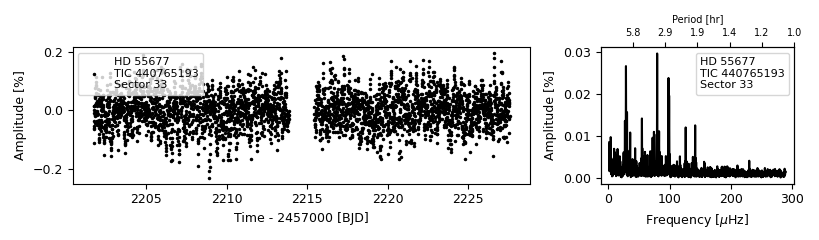
\includegraphics[width=0.9\linewidth]{figures/tic00000440765193_s033_flat1.fits.png}
    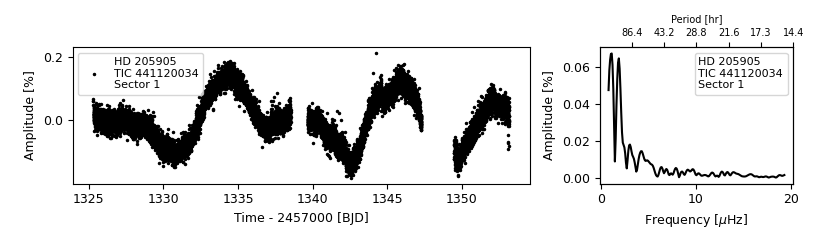
\includegraphics[width=0.9\linewidth]{figures/tic00000441120034_s001_normH.fits.png}
    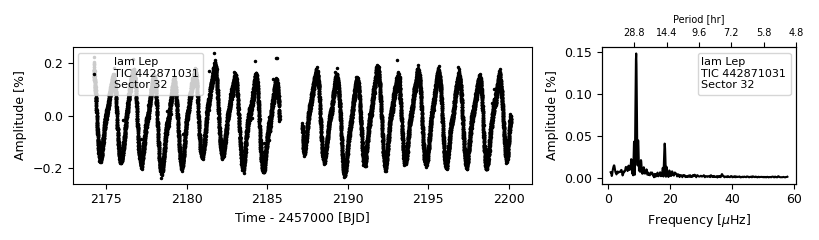
\includegraphics[width=0.9\linewidth]{figures/tic00000442871031_s032_norm1.fits.png}

    \caption{Light curve (left) and periodogram (right) of stars with significant detected variability. The \tess\ sector(s) used to generate both are labeled on each plot.}
    \label{fig:lcft2}
\end{figure*}

\begin{figure*}
    \centering

    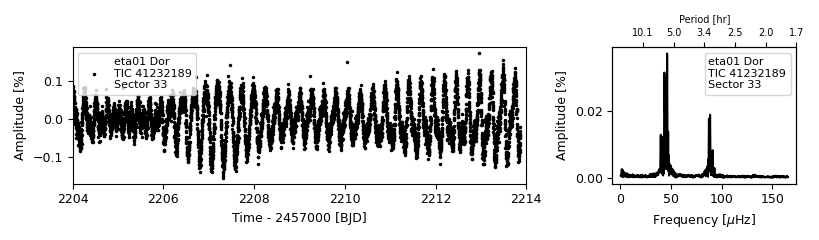
\includegraphics[width=0.9\linewidth]{figures/tic00000041232189_s033_norm1.fits}
    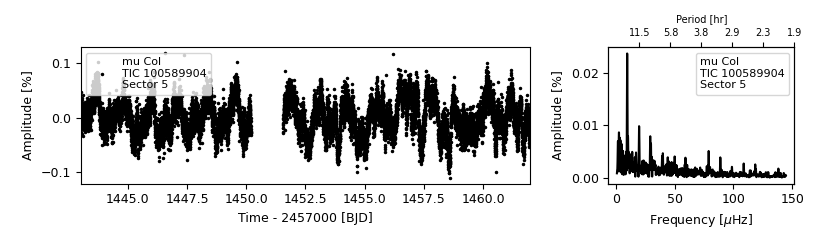
\includegraphics[width=0.9\linewidth]{figures/tic00000100589904_s005_norm1.fits}
    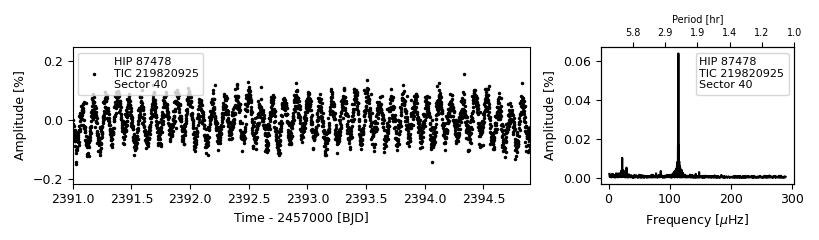
\includegraphics[width=0.9\linewidth]{figures/tic00000219820925_s040_norm1.fits.png}
    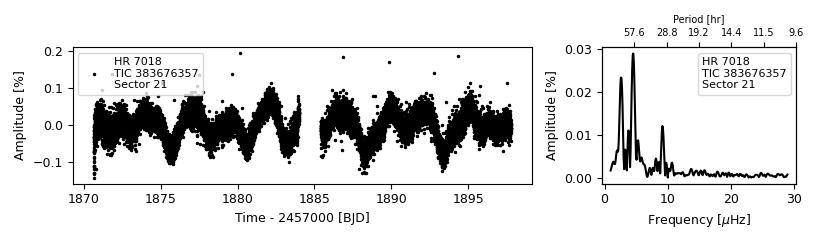
\includegraphics[width=0.9\linewidth]{figures/tic00000383676357_s021_norm1.fits.png}

    \caption{Light curve (left) and periodogram (right) of stars with significant detected variability. The \tess\ sector(s) used to generate both are labeled on each plot.}
    \label{fig:lcft3}
\end{figure*}
    
\begin{figure*}
\centering
    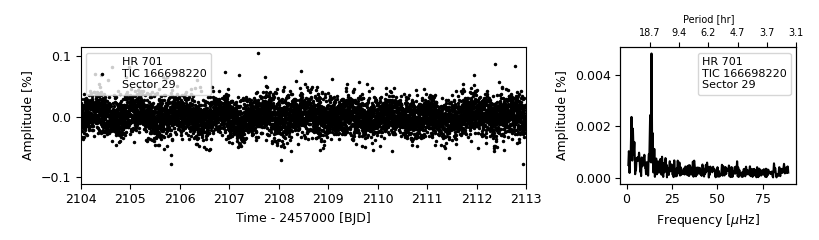
\includegraphics[width=0.9\linewidth]{figures/tic00000166698220_s029_norm1.fits}
    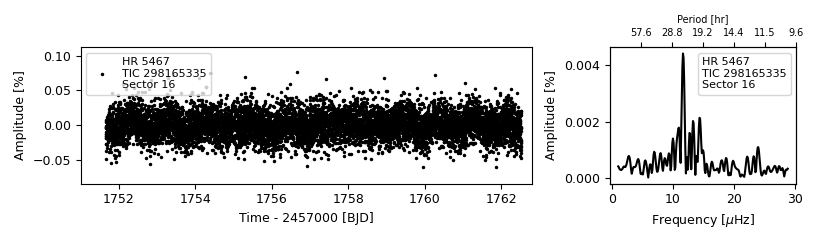
\includegraphics[width=0.9\linewidth]{figures/tic00000298165335_s016_norm1.fits.png}
    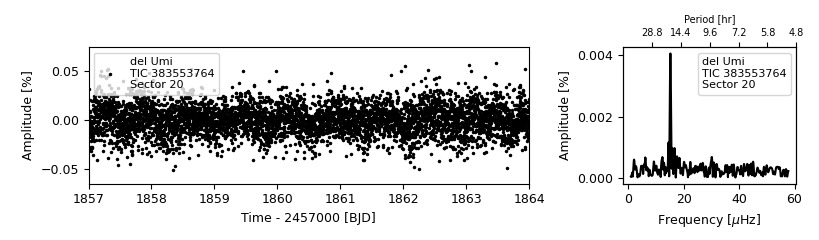
\includegraphics[width=0.9\linewidth]{figures/tic00000383553764_s020_flat2.fits.png}
    
    \caption{Light curve (left) and periodogram (right) of stars with significant detected variability. The \tess\ sector(s) used to generate both are labeled on each plot.}
    \label{fig:lcft4}
\end{figure*}


%How we looked for variability.
%Definition of any statistics we measured.

%%Create 1 Table with all the Results (star, TESS photometric limits, TESS <10day limits, T/F Variability detected)

\subsection{Not Observed to Vary}
\label{sec:novar}

We find no significant variability in 22 of the 37 stars we examined with existing \tess\ data. Figure~\ref{fig:novar} displays the light curves and periodograms for three well-known calibration stars with no significantly detected variability. We note that \tess\ commonly has large-amplitude systematic noise in its light curves at long periods, including noise at periods of 2~weeks due to the orbit of the spacecraft and near 1~day due to scattered light from the rotation of the Earth \citep{Luger2019}. Our sample of variable stars does not include those stars that only showed evidence of these types of systematic noise.


For those cases with no significant variability, we provide two statistics to better understand the upper limits of variability that could exist undetected in the \tess\ data in Table~\ref{tab:novar}. The photometric precision achieved by the \tess\ data is mostly driven by the brightness of the star, though in some cases systematic noise is playing a part. The $A^{max}_{<1d}$ is the maximum amplitude peak in the periodogram seen at periods less than 1 day. This statistic can serve as measure of the upper limit on consistent, short-period variability. $V_{99.7\%}$ can be interpreted as the largest peak-to-peak variation on time scales longer than 30-minutes that could be present in the data without detection. It is calculated by binning the light curve to 30-minutes and reporting the difference between the minimum and maximum relative flux for those points that lie within 99.7\% of the median observed flux. If the data is predominantly Gaussian noise, this value is approximately six times the size of the standard deviation of the light curve. For both of these statistics we report the sector that gives the smallest value, as some \tess\ sectors are noisier than others depending on scattered light from the Earth and Moon. 

\tess\ is able to provide limits to changes in brightness below 1\%  for all but six stars. These six stars are all dimmer than $12.9$\,mag in the \tess\ band.  For all but our dimmest star, \tess\ sees no evidence of coherent, periodic variability with amplitudes larger than 0.2\% for periods shorter than 1 day. Thus, \tess\ can still confirm the suitability as flux standards of many of the faintest sources in our sample.

\begin{deluxetable*}{llclcrr}
\tablecolumns{6}

\tablecaption{Upper limits on variability for those with no significant variations.}

\tablehead{
  \colhead{Name} & \colhead{TIC ID} & \colhead{Class} &\colhead{$T$} &\colhead{CROWD$^{\dagger}$} & \colhead{$A^{max}_{< 1d}$} & \colhead{$V_{99.7}$}\\
  \colhead{} & \colhead{} & \colhead{}& \colhead{[mag]} &\colhead{}& \colhead{[\%]}& \colhead{[\%]}
}
\startdata
GSPC P330-E &   8591766 &    G2V & 12.4 &    0.891 & 0.021 &  0.76 \\
   16 Cyg B $^*$ &  27533327 &    G3V &  5.6 &    0.630 & 0.017 &  0.21 \\
    HD 6538 &  39464221 &    G1V &  5.9 &    0.998 & 0.003 &  0.09 \\
     10 Lac & 128692445 &    O9V &  5.1 &    0.993 & 0.007 &  0.23 \\
   HD 37962 & 140282069 &    G2V &  7.2 &    1.000 & 0.002 &  0.09 \\
WD 1057+719 & 147921014 &  DA1.2 & 15.1 &    0.919 & 0.148 &  6.05 \\
      GD153 & 149505899 &    DA1 & 13.7 &    0.987 & 0.062 &  2.44 \\
  HD 116405 & 165370459 &    B9V &  8.4 &    0.969 & 0.003 &  0.10 \\
  HD 101452 & 181240911 &  A9mIV &  7.3 &    0.993 & 0.003 &  0.09 \\
   J1757132 & 219094190 &    A3V & 11.6 &    0.963 & 0.010 &  0.37 \\
 GSPC P041C & 219015049 &     G0 & 11.5 &    0.995 & 0.011 &  0.44 \\
 BD+60 1753 & 219752116 &    A1V &  9.7 &    0.992 & 0.006 &  0.17 \\
  HD 180609 & 229945862 &    A3V &  9.3 &    0.984 & 0.005 &  0.13 \\
  HD 115169 & 229980646 &    G2V &  8.7 &    0.984 & 0.003 &  0.11 \\
   J1802271 & 233067231 &    A3V & 12.0 &    0.963 & 0.023 &  0.82 \\
   J1805292 & 233075513 &    A1V & 12.2 &    0.965 & 0.014 &  0.49 \\
   J1743045 & 233205654 &    A5V & 13.3 &    0.986 & 0.032 &  1.32 \\
       GD71 & 247923021 &    DA1 & 13.4 &    0.788 & 0.055 &  1.90 \\
   G191-B2B & 327587572 &    DA0 & 12.2 &    0.903 & 0.021 &  0.74 \\
  HD 167060 & 365653206 &    G2V &  8.4 &    0.994 & 0.002 &  0.09 \\
GSPC P177-D & 417544924 &    G2V & 12.9 &    0.942 & 0.028 &  1.00 \\
 WD1657+343 & 471015233 &    DA1 & 15.8 &    0.631 & 1.289 & 37.88 \\
\enddata

\tablecomments{$^*$16 Cyg B is a known solar-type variable with low-amplitude modes (smaller than the limits reported here) at periods near 8 minutes (see \citealt{Metcalfe2012_16Cyg}). $A^{max}_{< 1d}$ is the maximum amplitude peak seen in the periodogram less than 1 day. $V_{99.7}$ is peak to peak flux change of those relative fluxes that lie within 99.7\% of the median flux.\\
$^{\dagger}$CROWD comes from the CROWDSAP estimate from the \tess\ SPOC pipeline and is the fraction of the flux that comes from the target star in the extracted aperture, as opposed to nearby sources in the TIC.}
\label{tab:novar}
\end{deluxetable*}
\vspace{-1em}
%\label{sec:novar}

\begin{figure*}
    \centering
    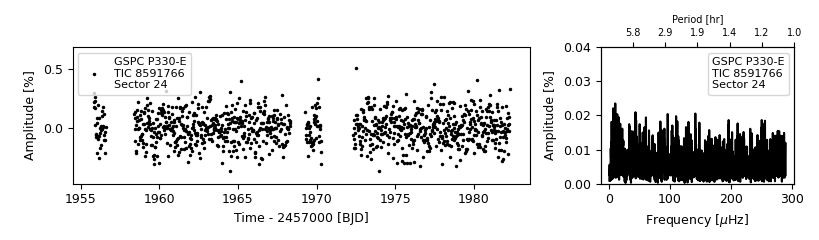
\includegraphics[width=0.8\linewidth]{figures/tic00000008591766_s024_flat2.fits.png}
    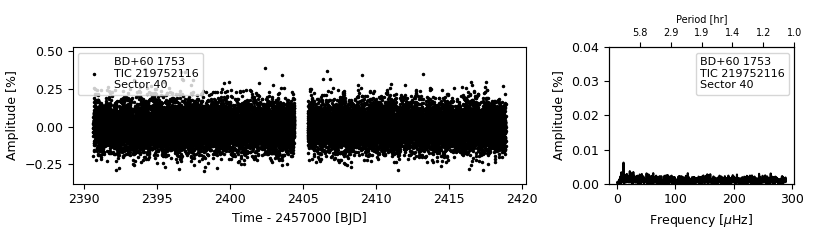
\includegraphics[width=0.8\linewidth]{tic00000219752116_s040_flat1.fits.png}
    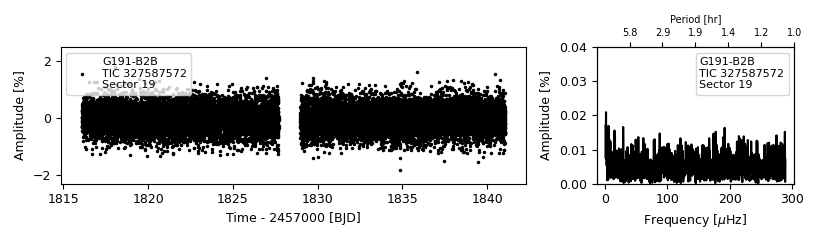
\includegraphics[width=0.8\linewidth]{figures/tic00000327587572_s019_norm1.fits.png}
    \caption{Light curves and Lomb-Scargle periodograms of three common calibration stars that show no significant, coherent variability in the \tess\ light curves.}
    \label{fig:novar}
\end{figure*}


% Jerzykiewicz et al. (2015) - 2015MNRAS.454..724J - no variability in 10 Lac

%We will have to keep picking standards and so TESS is a great resource.
% Discussion
% - Power of all-sky temporal surveys
% - Nature of variables
% - Predictions/speculation on wavelength dependence of variability

\section{Conclusions}
\label{sec:conclusion}

With its high-cadence, all-sky photometric survey of bright stars, \tess\ is a useful resource to vet potential spectrophotometric calibration stars for variability on time scale of a few minutes to a couple of weeks. Its precise relative photometry has allowed us to find peak-to-peak changes in flux as large as 1.4\% for 4 of the candidate calibrators for \webb. This variability appears to be caused by either stellar pulsations or stellar spots rotating in and out of view. At the same time, \tess\ relative photometry has set upper limits on optical to near IR brightness variability for most of the candidate standard stars at a level well below that needed to achieve the spectrophotometric requirements for \jwst. By identifying those with known issues, we provide the \webb\ calibration team with information necessary to pick those stars with the highest likelihood of accurate calibrations in the least amount of observing time. This work has already led to revisions of the \webb\ spectrophotometric calibration star list, see \citet{Gordon2022inprep}.

%the requirement to calibrate the instruments on \jwst\ to an accuracy better than 2\% \citep{jdox}.  

%The variability of a candidate is only one consideration among many when choosing the best candidates for calibration. The \webb\ calibration program \citep{Gordon2022inprep} will be based on observations of many calibration stars to ensure that the calibration does not  hinge on one star acting as expected. By identifying those with known issues, we provide the \webb\ calibration team with information necessary to pick those stars with the highest likelihood of accurate calibrations in the least amount of observing time.

%Those stars with variations in flux larger than $\approx$1\% could create unnecessary systematic noise when trying to accurately calibrate the telescope. Not only would variability introduce random photometric errors, but it could also reveal a number of other issues that would make models of a star less reliable.  For example, variability due to stellar rotation, while a problem in itself, could also reveal strong magnetic fields and star spot activity, which could render models of the star inaccurate --- most notably, star spots cause multiple temperature components at the photosphere, severely complicating simple modeling.   

Some of the stars vetted in this paper are the same stars that were used to calibrate telescopes such as Spitzer \citep{Reach2005} and Hubble \citep{Bohlin2011AJ}, and some may be used to calibrate future space and ground-based telescopes.  Because \tess\ is an ongoing all-sky survey, in the future \tess\ will serendipitously continue to monitor many of the \webb\ spectrophotometric calibration stars. Continuous monitoring by \tess\ will inform us if the star changes in brightness in new or unexpected ways.  Some of these observation may even be contemporaneous with the \webb\ calibration observations, as both missions plan to be operating at the same time.  This work provides further evidence that small NASA missions like \tess\ can provide crucial supporting observations which enable larger missions like \jwst\ to accomplish their science goals.

\begin{acknowledgments}
%\textcolor{red}{Please add your acknowledgements here.}
This paper includes data collected by the \tess\ mission. Funding for the \tess\ mission is provided by the NASA's Science Mission Directorate. We thank the STScI internship program and \jwst\ for providing funding for for MK. JJH acknowledges financial support through NASA Award 80NSSC20K0592.
This research has made use of the VizieR catalogue access tool, CDS, Strasbourg, France (DOI: 10.26093/cds/vizier). The original description of the VizieR service was published in A\&AS 143, 23.
This research has been made possible by the MAST archive for access to the \tess\ light curves, \tess\ Input Catalog, and target pixel files.
\end{acknowledgments}

\vspace{5mm}
\facilities{TESS, JWST, MAST}

\software{astropy \citep{astropy2013,astropy2018},  
          lightkurve \citep{lightkurve},
          TESS\_Localize \citep{HiggensBell}
          }

\bibliography{references}{}
\bibliographystyle{aasjournal}

\end{document}


%THIS PARAGRAPH IS REDUNDANT WITH THE INTRO BUT SAYS A BIT MORE.  SOME OF THE TEXT MAY BE USEFUL IN THE DISCUSSION.  Each candidate must be vetted for any signs of trouble, and one important indicator is variability.  Not only would variability introduce random photometric errors to the assumed truth spectrum, but it could also point to a number of other issues that would make models of a star less reliable.  For example, periodic eclipses are the most straightforward way to reveal an unseen companion, but variability can also result from more subtle orbital interactions.  Stellar pulsation, especially for A dwarfs, is another concern.  Variability due to stellar rotation, while a problem in itself, could also reveal strong magnetic fields and starspot activity, which could render models of the star inaccurate.

%Calibrations of \webb's instruments is done through both observations of stars and models of the stellar flux density. Calibration stars are chosen to be those where the spectra can be modeled to the 1\% level. \webb\ has chosen a set of A, G and white dwarf stars that have been observed by both \textit{Hubble} and \textit{Spitzer} \citep{Krick2021IRAC} to do these calibrations and require that at least 4~stars that can be modeled to the required accuracy in order to calibrate all the observing modes of the \webb\ observatory.  


%class are generally associated with spectral classes from late A to early F. Here we present \webb\ standards, which generally fall in the range A0--A3, however,  here we find multiple occurrences of $\delta$ Scuti stars and $\gamma$ Dor stars, indicating that the spectral classification may not be accurate.

%Two classes of variables have properties similar to the four variable A dwarfs in the standard-star sample:  $\alpha^2$ CVn and rapidly oscillating Ap (roAp) stars.  The $\alpha&2$ CVn variables have periods between half a day or so up to $\sim$ days, amplitudes of 0.1 mag or less, spectral classes of B9--A5, and spectral types indicating peculiarities, with a suffix ``p'' and other descriptors indicating strong lines from Si, Sr, Cr, and/or rare earths like Eu \citep{Pettit1987, Hoffmeister1984}.  High-resolution spectra reveal strong magnetic field lines, and their variability is linked to the rotation of spots.

%The roAp stars, discovered by \cite{Kurtz1982} show similar spectral properties.  Recent TESS observations have increased the sample of roAp stars to a total of 88 \citep{Holdsworth2021}.  The spectral classes cover a wider range, from early A to late F.  Like the $\alpha^2$ CVn stars, the amplitudes are generally small, but the roAp stars can show longer periods due to rotation and shorter periods due to non-radial pulsations.

%also pulsations, spots and rapid pulsations which occur in rapidly oscillating Ap (roAp) stars \citep{Kurtz1978,Kurtz1982}. For roAp stars, the pulsations, which have periods on between 4.7--6\,min\citep{Holdsworth2021}, are not the dominant feature in the light curve. Like many peculiar A (Ap) stars, roAp stars have prominent spots, which can generate variations on the order of magnitudes. However, these variations tend to be more prominent in roAp stars due to their strong magnetic fields, which have been measured up to 34\,kilogauss \citep{Mathys2017}.

%Kaye1999 - Kaye, A.~B., Handler, G., Kriscinuas, K., et al.\ 1999, \pasp, 111, 840.
%Hoffmeister, C., Richter, G., \& Wenzel, W., Variable Stars, 1984 (Berlin: Springer-Verlag)

%The four A dwarfs identified with peak-to-peak variability of 0.4\% or more have periods and spectral classes that resemble the $\alpha^2$ CVn and roAp stars, although their amplitudes tend to be smaller and their spectral classifications have not noted any of the expected peculiarities.  HR 6514 has a spectral type of A4 V \citep{Crowley1969}, but otherwise could be a low-amplitude roAp star.  J1812095, with its longer 2.4-day period, looks more like a low-amplitude $\alpha2$ CVn variable.  The other two variable A dwarfs, J1732526 and J1808347, have periods of 0.5--0.6 h and amplitudes of 1.4--1.6\% and could be roAp stars.

%These last three stars, J1812095, J1732526, and J1808347, were selected as \webb\ candidate stars because they were used as standards by IRAC on Spitzer \citep{Reach2005}.  J1812095 was one of 11 primary standards for IRAC during the cryogenic mission.  The low amplitude of its variability would have been difficult to detect with IRAC.  All three stars have rather ordinary spectral types not at all like what would be expected for $\alpha^2$ CVn or roAp variables, but their spectral types were determined photometrically, not spectroscopically (W.\ Reach, private communication, 2005).  The spectral types were assigned based on the spectral type of stellar templates which best fit the available photometry prior to the Spitzer mission.  It would be worthwhile to investigate the optical spectra of these low-amplitude variables with sufficient spectral resolution to search for the expected unusual properties.

% HR 6514 P = 0.054 d = 1.3 h, V95 = 0.42%
% J1812095 P = 2.44 d, V95 = 1.57%
% J1732526 P = 0.020 d = 0.5 h, V95 = 1.40%
% J1808347 P = 0.026 d = 0.6 h, V95 = 1.65%

%NOT SURE HOW TO FIT THE FOLLOWING INTO THE NARRATIVE.

%RoAp stars are primarily thought to pulsate via the $\kappa$ mechanism, also known as the heat engine mechanism, although alternative mechanisms have been proposed for the highest frequency pulsations \citep{Cunha2013}. Like roAp stars, $\delta$ Scuti stars also pulsate via the Kappa mechanism, although their pulsation periods are 18\,min--8\,hr \citep{Amado2004}. They pulsate in radial and non-radial pressure modes and low-order gravity modes, with their flux variations reaching 0.9\,mag.

%..\textcolor{red}{Please write about astrophysics here and include in the per star bit.}


%The 1$\sigma$ variability is under 0.1\%, and like HR~6514, does not by itself disqualify this star as a standard.  $\lambda$ Lep is one of the hot B dwarfs under consideration for use as standards starting in \jwst\ Cycle 2.

% Burssens et al. (2020) - 2020A&A...639A..81B - find periods of 1.26 and 0.63 days
% use Lesh 1968 for sp type ref